\documentclass[times, 10pt,dvipdfmx]{jsarticle}
\usepackage{graphicx}  
\usepackage{times}
\usepackage[most]{tcolorbox}
\usepackage{ascmac}
%\usepackage{amsmath}
\usepackage{amsmath,amssymb}
\usepackage{fancybox} 
\usepackage{version}
\usepackage{mdframed}
\usepackage{url}
\usepackage{xcolor}
%\usepackage{chapterbib}
\usepackage{tboxit}
\usepackage{boxedminipage}
\usepackage{rdbkbox}
\usepackage{bm}
\usepackage{qexam}
\usepackage{multienum}
\usepackage{version}
\usepackage{caption}
\makeatletter
\renewcommand{\figurename}{図}
\renewcommand{\tablename}{表}
\renewcommand{\refname}{References}
%\def\theequation{\thesection.\arabic{equation}}
%\def\thefigure{\thesection.\arabic{figure}}
%\def\thetable{\thesection.\arabic{table}}
\@addtoreset{equation}{section}
\@addtoreset{figure}{section}
\@addtoreset{table}{section}
\makeatother 
\setlength{\oddsidemargin}{0mm}
\setlength{\evensidemargin}{0mm}
\setlength{\textwidth}{16cm}
\newtheorem{kadai}{Exercise}[section]
\newtheorem{tisiki}{Advanced}[section]
\newtheorem{reidai}{Example}[section]
\newenvironment{kaisetsu}
{\vspace{5mm}\begin{center}\dotfill Explanation \dotfill\end{center}}
{\begin{center}\dotfill EoE \dotfill\end{center}\vspace{5mm}}
\newenvironment{theorem}%
{\begin{mdframed}[backgroundcolor=lightgray,linewidth=0]}%
{\end{mdframed}}
\newenvironment{advanced} 
{\vspace{5mm}\begin{center}\Dotfill \\
\Dotfill Advanced Study \Dotfill\end{center}}
{\begin{center}\Dotfill End of Advanced Study \Dotfill \\
\Dotfill 
\end{center}\vspace{5mm}}
\definecolor{Gray}{gray}{0.85}
\excludeversion{kaisetsu}
\tcbset{
    frame code={}
    center title,
    left=0pt,
    right=0pt,
    top=0pt,
    bottom=0pt,
    colback=gray!70,
    colframe=white,
    width=\dimexpr\textwidth\relax,
    enlarge left by=0mm,
    boxsep=5pt,
    arc=0pt,outer arc=0pt,
    }
%
%
%
%
\DeclareMathOperator*{\argmax}{argmax}
\newcommand{\figSize}{0.7}
\newcommand{\hhline}{\begin{center}\begin{tabular}{c}\hline\hline\end{tabular}\end{center}}
\newcommand{\ffbox}[1]{\centerline{\vspace{1cm}\fbox{\parbox{0.8\textwidth}{#1}}\vspace{1cm}}}
%\newcommand{\ffbox}[1]{{\vspace{1cm}\fbox{\parbox{1.0\textwidth}{#1}}\vspace{1cm}}}
\newcommand{\ftbox}[2]{\vspace{5mm}\tboxit{#1}{\vbox{\hsize 0.8\textwidth #2}}}
%\newcommand{\bm}[1]{\boldmath{#1}}
%\renewcommand{\dotfill}{\vspace{10mm}\dotfill}
\setlength{\textheight}{630pt}
\newcommand{\obox}[1]{\vspace{5mm}\ovalbox{#1}}
\newcommand{\vs}{\vspace{5mm}}
\newcommand{\ah}{\vspace{8cm}}
\newcommand{\anscol}{\underline{\hspace{6cm}}}
\newcommand{\ahd}{\vspace{10cm}}
\newcommand{\dia}{\vspace{3cm}\centering{$\diamond$ \hspace{1cm} $\diamond$ \hspace{1cm} $\diamond$}\vspace{3cm}}
\usepackage{fancybox}
\newtheorem{prog}{program}[section]
\newenvironment{program}
{
  \VerbatimEnvironment
  \baselineskip=.40\normalbaselineskip
  \begin{Verbatim}
}
{
  \end{Verbatim}
  \baselineskip=\normalbaselineskip
  \noindent
}
%%\newcommand{\na}{\begin{quote}\setlength{\baselineskip}{12pt}\begin{verbatim}}
%\newcommand{\ea}{\end{verbatim}\end{equote}}
%\newenvironment{FRAME}{\begin{trivlist}{\item[]
%\hrule
%\hbox to \linewidth\bgroup
% \advance\linewidth by -30pt
% \hsize=\linewidth
% \vrule\hfill
% \vbox\bgroup
% \vskip15pt
%  \def\thempfootnote{\arabic{\mpfootnote}}%
%  \begin{minipage}{\linewidth}}{%
%\end{minipage}\vskip15pt
%\egroup\hfill\vrule
%\egroup\hrule
%\end{trivlist}}
\excludeversion{answer}\includeversion{solspace}
\pagestyle{plain}
\begin{document}
\begin{center}
{\Large DS1　微分・積分　最終試験}
\vspace{4cm}
\ffbox{
\begin{itemize}
\item 時間は70分。
\item 記述問題を除き答えを下線がある欄に記入し、導出経緯をその下に書く。
\item 資料持ち込み可能。ネットで調べてもよいが、質問して答えやヒントをもらってはいけない。生成AIに聞くのも本テストでは禁止。
\item 導出経緯を解答欄に収まる範囲で詳しく書くこと。欄が足りなくなる場合には、最後の余白ページに問題番号を明記して、解答欄から「page 13に続く」などと参照すること。原則として解答欄だけの記入に得点は与えられない。
\item 表計算ソフトを使う、プログラムを書くなどしてコンピュータで答えを求めてもよい。その場合、答えのみでなく、手順概要を記載すること。
\item 学生証を机の上に出す。
\item (1)-(10)が5点、 (11)-(15)が10点の100点満点。
\end{itemize}
}
\vspace{2cm}

{２０２５年７月２１日}\\
%{担当教員：三次　仁}
\vspace{2cm}

\begin{tabular}{p{2cm}p{5cm}}
学籍番号: &\underline{\hspace{8cm}} \\
& \\
& \\
氏名 : &\underline{\hspace{8cm}}\\
\end{tabular}


\end{center}
\clearpage
%\begin{qlist}
%\qitem 48と124の最大公約数と最小公倍数を求めよ

%\vspace{5mm}
%最大公約数\underline{\hspace{3cm}} 最小公倍数\underline{\hspace{3cm} }
%\ah
%\end{solspace}
% \qitem 1147と1517の最大公約数と最小公倍数を求めよ%
 % \begin{qlist2}
  %  \qitem 最大公約数はいくつか
   % \qitem 最小公倍数はいくつか
 % \end{qlist2}
   %\qitem 356と623と1424の最大公約数と最小公倍数を求めよ
   
%\vspace{5mm}
%最大公約数\underline{\hspace{3cm}} 最小公倍数\underline{\hspace{3cm} }
%   \ah
%%\end{qlist}
\begin{qlist}
\qitem $\cos(4x)=8\cos^4(x) - 8\cos^2(x) + 1$となることを加法定理を用いて示せ。
\ah
\end{qlist}
%\begin{qlist}
%\qitem 極限を求めよ。極限が求められない場合にはその理由を説明せよ。
%\begin{equation}
%\lim_{x \to 2} \frac{x^2-3x +2}{x-2} \nonumber 
%\end{equation}

%\vspace{5mm}%
%極限\underline{\hspace{3cm}} 
%\ah
%\end{qlist}
\begin{qlist}
\qitem 極限を求めよ。極限が求められない場合にはその理由を説明せよ。
\begin{equation}
\lim_{x \to 0} x (\log_e (x))^2  \qquad   x > 0 \nonumber
\end{equation}

\vspace{5mm}%
極限\anscol
\ah
\end{qlist}
\begin{qlist}
\qitem 極限を求めよ。極限が求められない場合にはその理由を説明せよ。
\begin{equation}
\lim_{n \to \infty}  n^{-\frac{3}{2}} \sum_{i=1}^n \sqrt{i}  \nonumber 
\end{equation}

\vspace{5mm}%
極限\anscol
\ah
\end{qlist}
%\begin{qlist}
%\qitem 極限を求めよ。極限が求められない場合にはその理由を説明せよ。
%\begin{equation}
%\lim_{x \to 2} \frac{x^2-x-2}{x^3 - 7}  \nonumber
%\end{equation}
%
%\vspace{5mm}%
%極限\underline{\hspace{3cm}} 
%\ah
%\end{qlist}
\begin{qlist}
\qitem 極限を求めよ。極限が求められない場合にはその理由を説明せよ。
\begin{equation}
\lim_{x\to 0} \left(1+x\right)^\frac{1}{x} \nonumber 
\end{equation}

\vspace{5mm}
極限\anscol
\ah
\end{qlist}
\begin{qlist}
    \item 以下の極限を求めよ。極限が求められない場合にはその理由を説明せよ。
    \begin{equation}
        \lim_{x\to 0} \frac{\sin(x) - x}{x^3} \nonumber 
    \end{equation}
    
\vspace{5mm}
極限\anscol
\ah
\end{qlist}
\begin{qlist}
\qitem 次の$y$を$x$で微分せよ
\begin{equation}
y = \frac{x^2}{x^3-1} \qquad  x \neq 1\nonumber
\end{equation}

\vspace{5mm}
$\frac{dy}{dx}=$\anscol
\ah
%\qitem 次の$y$を$x$で微分せよ
%\begin{equation}
%y = e^{2x+4} \nonumber
%\end{equation}
%\vspace{5mm}
%$\frac{dy}{dx}=$\anscol
%\ah
%\clearpage
\qitem 次の$y$を$x$で微分せよ
\begin{equation}
y = x{\tan{(x)}}\nonumber 
\end{equation}

\vspace{5mm}
$\frac{dy}{dx}=$\anscol
\ah
\end{qlist}
\begin{qlist}
\qitem 次の式が成立することを証明せよ

\begin{equation}
\arctan({\sqrt{2}x -1}) - \arctan({\sqrt{2}x + 1})  = \arctan({x^2}) + \frac{\pi}{2}  \nonumber
\end{equation}
\ah

\end{qlist}
%\begin{qlist}
%\qitem 次の$y$を$x=0$近傍で$x$の二次式で近似せよ。
%\begin{equation}
%y = \tan{(x)} \nonumber 
%\end{equation}
%\ah
%\begin{qlist}
%\qitem 次の$z$を$(x,y)=(0,0)$近傍で、$x,y$の二次式(斉次式）で近似せよ
%\begin{equation}
%z = \cos(x)\cos(y) \nonumber 
%\end{equation}
%
%\vspace{5mm}
%$z=$\anscol
%\ah
%\end{qlist}
%\clearpage
\begin{qlist}
\qitem 不定積分せよ
\begin{equation}
\int x^{\frac{3}{2}} \log_e(x) dx \nonumber 
\end{equation}

\vspace{5mm}
$\int x^{\frac{3}{2}} \log_e(x) dx =$\anscol
\ah
\end{qlist}

%\begin{qlist}
%\qitem $a>0$で、$x,y$が媒介変数$\theta$で以下のように書けるとき
%\begin{eqnarray}
%x &=& a\theta - a\sin\theta \nonumber \\
%y &=& a - a\cos\theta \nonumber 
%\end{eqnarray}
%$\theta$が0から$2\pi$まで変化した時の曲線の長さ$I$を求めよ。
%
%\vspace{5mm}
%$I=$\anscol
%\ahd
%\end{qlist}
\begin{qlist}
\qitem 
以下の陰関数$f(x,y)$について$ y\geqq 0$の範囲における面積を求めよ。
\begin{equation}
f(x,y) = 9(x-2)^2 + y^2 - 9  = 0　 \nonumber
\end{equation}

\vspace{5mm}
面積 \anscol
\ah
\end{qlist}
\clearpage
\begin{qlist}
%\qitem
%%$(x,y) = (2,0)$を中心として、
%\begin{equation}
%\left(\frac{x-2}{2}\right)^2 + y^2 = 1 \nonumber
%\end{equation}
%で与えられる楕円を$y$軸周りに回転してできるトーラスの体積$V$を求めよ。
%
%\vspace{5mm}
%$V=$ \anscol
%\ahd
%\clearpage
\qitem $ 0 \leqq x \leqq 1$の範囲で$y = x^4$の関数を$y = x$を軸として回転させてできる立体の体積$V$を求めよ。

\vspace{5mm}
$V=$ \anscol
\ahd
\clearpage
%\qitem  $4(y-3)^2 + x^2 = 4$の陰関数を$x$軸周りに回転してできる立体の体積を求めよ。
%\begin{figure}[h]
%\centering
%\includegraphics[width=5cm]{torusint.eps}
%\end{figure}
%\begin{qlist}




%\qitem 領域$D$で重積分せよ。$\iint_D xy dxdy \qquad D: (x-2)^2+ y^2 \leqq 4 \quad y \geqq 0$
%
%\vspace{5mm}
%積分値 \anscol
%\ahd
\qitem $|x|$を$x$の絶対値とした場合、$f(x,y) = |x|+|y|$に対して$x^2 - 2x + y^2 = 0 $の拘束条件で$f(x,y)$が極値となる$x,y$とその極値を求めよ。複数ある場合には、極限を与える$x,y$と極限値が対になるように解答すること。

\vspace{5mm}
\begin{tabular}{p{5cm}p{7cm}} 
極限を与える$(x,y)$  &  \underline{\hspace{8cm}} 
\end{tabular}

\vspace{1.5cm}
\begin{tabular}{p{5cm}p{7cm}} 
極値 & \underline{\hspace{8cm}} 
\end{tabular}
\ahd

%\vspace{5mm}
%体積\underline{\hspace{5cm}}
%\ahd
\end{qlist}
\clearpage

\begin{qlist}
\qitem $f(x) = \sin(\frac{1}{x})$を$x= \frac{1}{\pi}$においてテイラー展開し、$x = \frac{1}{\pi} + h$として$h$の三次多項式で近似せよ。
\vspace{5mm}

$f(\frac{1}{\pi} +h) \approx$ \underline{\hspace{10cm}}
\ahd
\end{qlist}


\clearpage

%\begin{qlist}
%\qitem $e$をネイピア数として次の式を定積分せよ。
%\begin{equation}
%I = \int_{-\infty}^{\infty} e^{(-r^2)}  dr \nonumber
%\end{equation}
%
%\vspace{5mm}
%積分値 \underline{\hspace{3cm}}
%\ahd
%\qitem $|x|$を$x$の絶対値とした場合、$z = |x|+|y|$に対して$x^2 - 2x + y^2 = 0 $の拘束条件で極値を与える$x,y$とその極値を求めよ。
%複数ある場合には、極限を与える$(x,y)$と極値が対になるように解答すること。
%
%\vspace{5mm}
%極限を与える$(x,y)$ \underline{\hspace{6cm}} 極値\underline{\hspace{6cm}}
%\ahd
%\end{qlist}
\clearpage
\begin{qlist}
\qitem 表\ref{tab:covid}は厚労省公開データ（https://www.mhlw.go.jp/stf/covid-19/open-data.html)から抜粋した,
ある時期の新型コロナ新規感染者数データである。８個あるデータの組を東京都における感染者数$x_i$と同時期の全国感染者数$y_i$の組と考え、このデータから東京都の感染者数$x$と全国感染者数$y$の関係を$y=ax+b$の一次式を用いて最小二乗誤差$L$を最小にする場合の$a$, $b$を計算し、小数点１位（千人）までの有効数字で示せ。
\begin{equation}
L = \sum_{i=0}^7 (y_i -y )^2 \nonumber
\end{equation}


\vspace{5mm}
$a$= \underline{\hspace{3cm}}  $b=$\underline{\hspace{3cm}}
\begin{table}[h]
\centering
\caption{新型コロナ新規感染データ（単位万人)}
\label{tab:covid}
\begin{tabular}{rrr}
\hline
時期 & 東京 & 全国 \\
\hline 
22年5月 & 10	& 96\\
22年6月 & 5	& 47 \\
22年7月 & 51	& 309 \\
22年8月 & 81	& 640 \\
22年9月 & 27	& 272 \\ 
22年10月 & 10	& 105 \\
22年11月 & 20	& 206 \\
22年12月 & 42	& 403 \\
%23年1月 & 371621	& 4128277 \\
%23年2月 & 78889	& 1038622 \\ 
%23年3月 & 24390	& 307812 \\
%23 年5月 & 29419	& 229863 \\
\hline
\end{tabular}
\end{table}
\clearpage


\qitem　$x_i, y_i$からなる観測データ（$  0 \le i \le N-1$）の組を用いて、dataを0と1に二分類することを考える。図\ref{fig:sig}に示すように、観測データの$x_i, y_i$については、その組み合わせがdata=0を表しているのか、それともdata=1を表しているのか、の正しい分類$c_i$（ラベル）はわかっているとする。つまり$c_i=0 \; \textrm{or} \; 1$である。無線で受信したデジタルデータを受信器で0か1に分類するイメージである。

\begin{figure}[h]
\centering
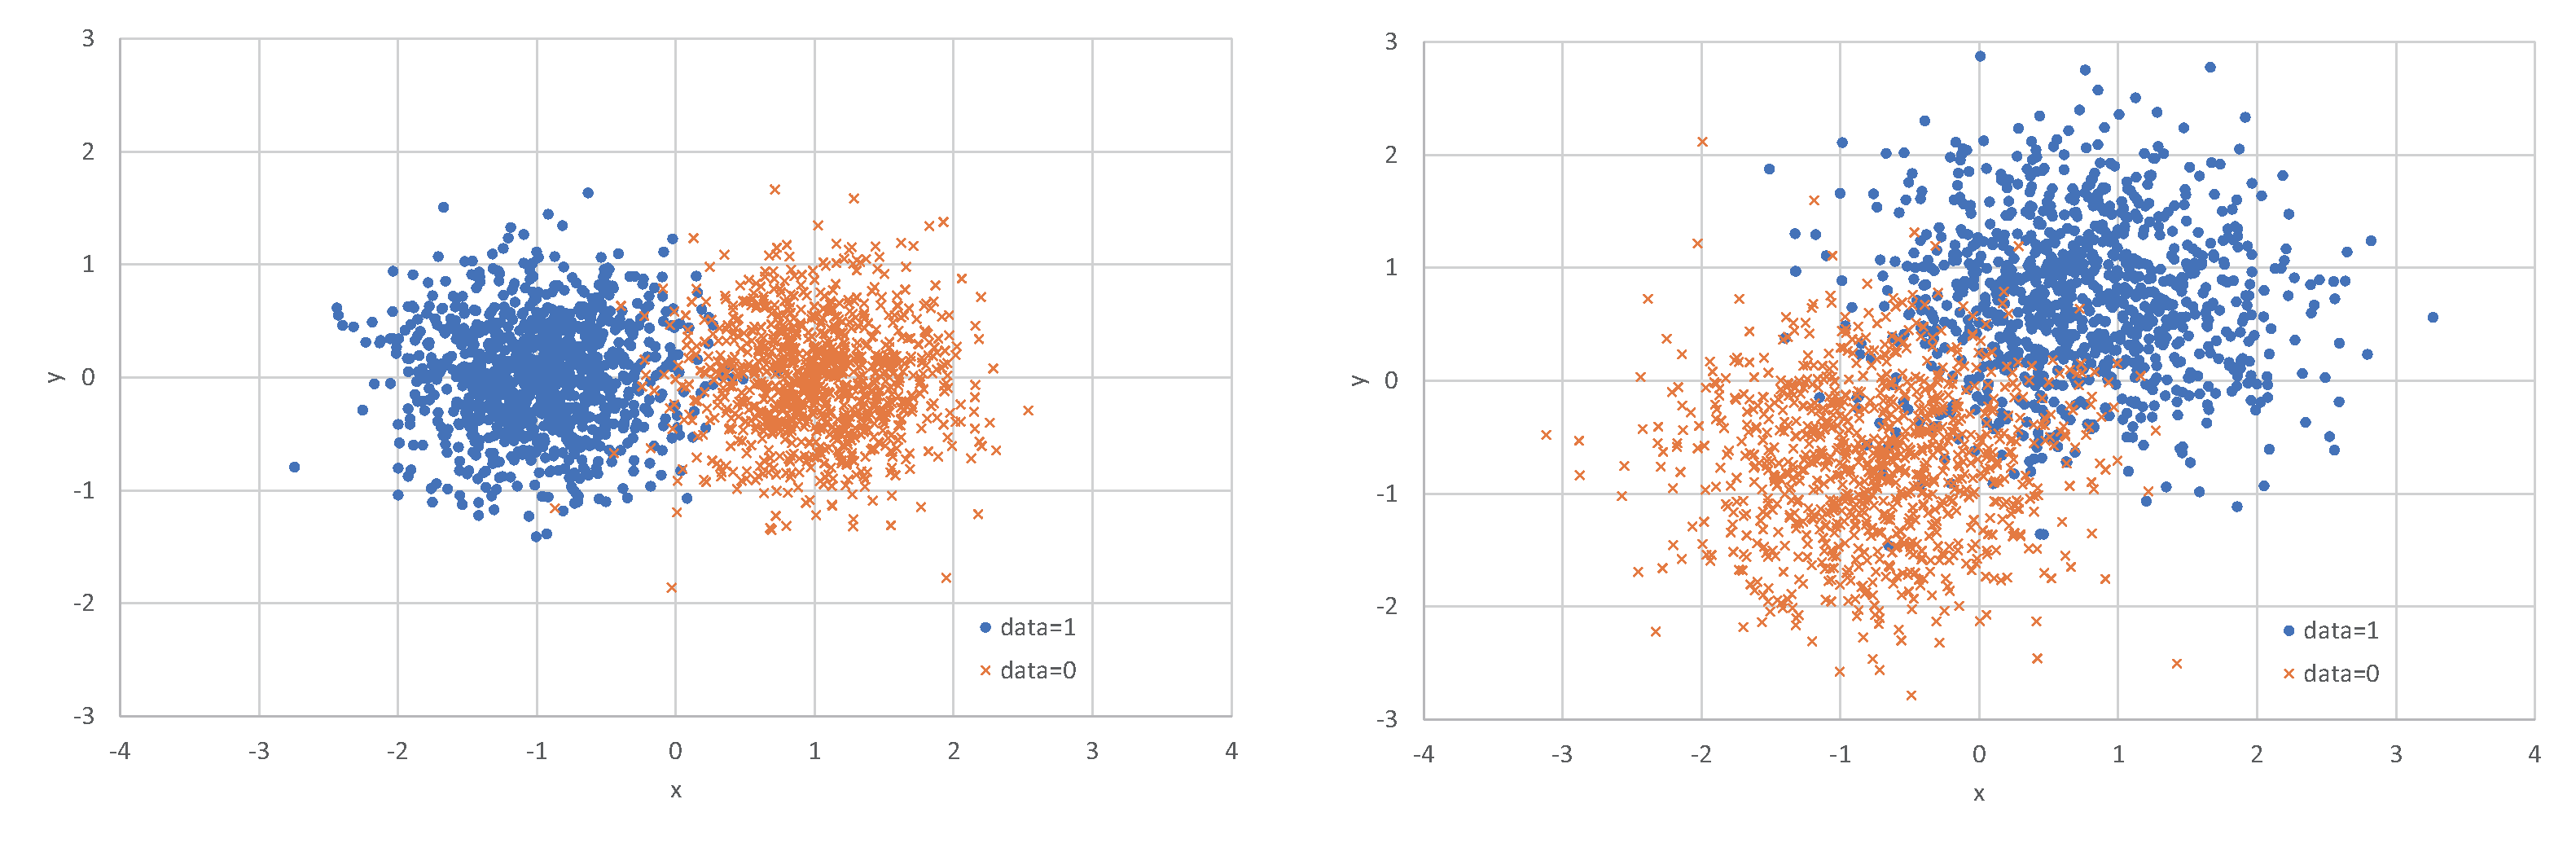
\includegraphics[width=12cm]{sig.eps}
\caption{観測データをdata=0, data=1に分類する. 観測データは時と場合によっては上記のように分布が異なるが、それぞれのラベルは既知である}
\label{fig:sig}
\end{figure}
観測外のデータの組に対しても$c_i=0 \; \textrm{or} \; 1$のいずれかに分類する分類器を観測データから作るために、未知の２つの係数$w_x, w_y$を用いて、以下の関数$p_i$を定義する。$e$はネイピア数である。
\begin{equation}
p_i =  \frac{1}{1 + e^{-(w_x x_i + w_y y_i)}} \nonumber
\end{equation}
表記を簡単にするために$\chi_i = w_x x_i + w_y y_i $を導入すると、$p_i$は以下となる。
\begin{equation}
p_i =  \frac{1}{1 + e^{-\chi_i}} \nonumber
\end{equation}

%この$p_i$が,ラベルが$c_1$である確率であるなら、$w_x, w_y$を決定することを考える。


以下の問に答えよ。

\begin{enumerate}
\item $\chi_i= w_xx_i+w_yy_i$を横軸に、$p_i$を縦軸にしてグラフを書くとどのような形になるか。下の座標軸に切片や極限値をできるだけ明確にして書け。
\begin{figure}[h]
\centering
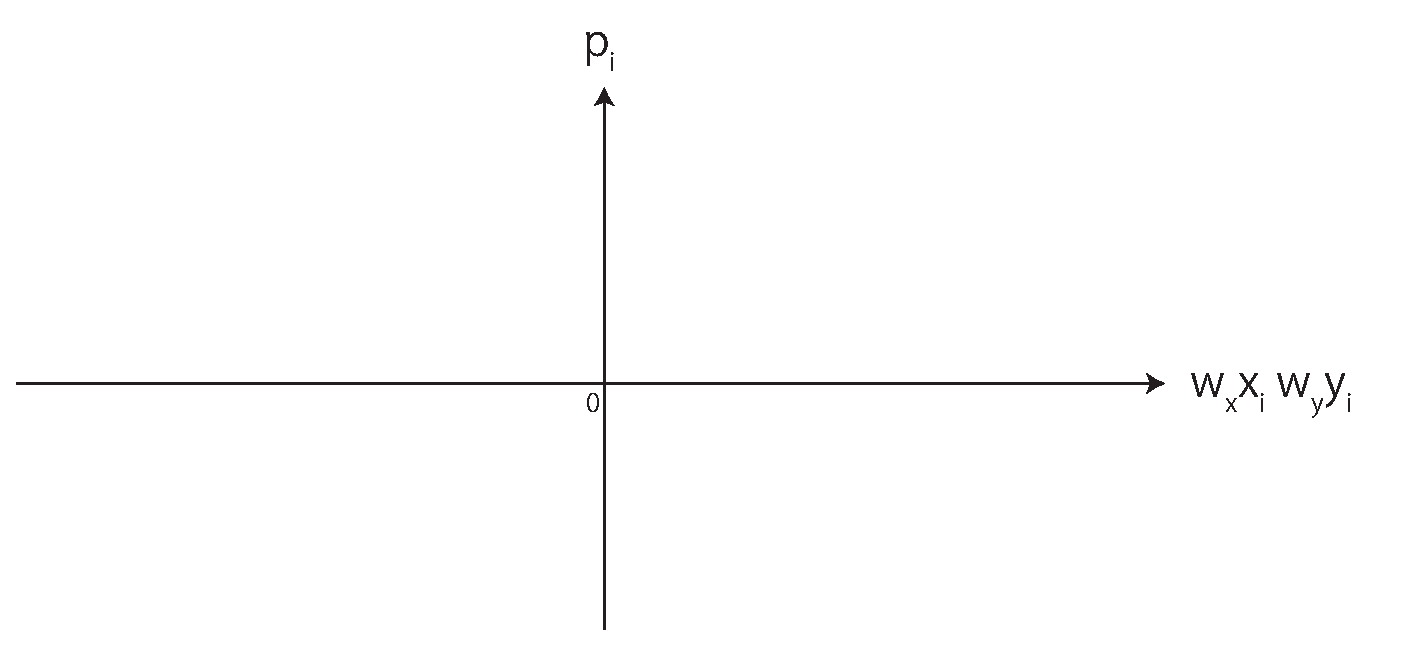
\includegraphics[width=10cm]{siggraph.eps}
%\caption{観測データをdata=0, data=1に分類する}
%\label{fig:sig}
\end{figure}
\clearpage
\item $x_i, y_i$の組がデータ1である確率を$p_i$で表す時、逆にその組がデータ0である確率は$1-p_i$となる。
$N$組の観測データ$w_x, w_y$を用いて$L$を次のように定義する。$c_i$は0か1のいずれかなので、$\log_e{p_i}$、$\log_e{(1-p_i)}$のどちらかがラベルに応じて総和されることになる。
\begin{equation}
L(w_x, w_y) = \sum_{i=0}^{N-1} c_i \log_e{p_i} + (1-c_i) \log_e{(1-p_i)}　\nonumber \label{eq:loss}
\end{equation}
この$L$を最大にする、つまり$\frac{\partial L}{\partial w_x}=0, \frac{\partial L}{\partial w_y}=0$を与える$w_x, w_y$が求める解である。
\footnote{$L$は観測データの結合確率を対数表示した対数結合確率である。偏微分により、対数結合確率の極大値を求めることができる。}



$\frac{\partial L}{\partial w_x}$と$\frac{\partial L}{\partial w_y}$を$x_i, y_i, c_i, p_i$を用い、できるだけまとめて記述せよ。

\vspace{10mm}
$\frac{\partial L}{\partial w_x} =$\underline{\hspace{8cm}}  \\

\vspace{5mm}
$\frac{\partial L}{\partial w_y}=$\underline{\hspace{8cm}}
\ahd


\end{enumerate}


\end{qlist}
\newpage
%\thispagestyle{empty}
\mbox{}
\newpage
\mbox{}
\newpage
\mbox{}
\newpage
\mbox{}
\end{document}
 